\chapter[Introduction]{Introduction\footnote{Portions of this thesis appeared in the following publication: Bandi, V and Gutwin, C. 2020. Interactive Exploration of Genomic Conservation. In Proceedings of Graphics Interface 2020 (GI ’20). To appear. DOI=doi.org/xx.xx/xxxx.xxxxx}}

With the emergence of new sequencing systems, genomic data is being generated at an unprecedented rate. Almost two decades back, \textit{The Human Genome Project} took 13 years and over \$3 billion dollars to sequence the entire human genome whereas the same information can be sequenced today in under an hour for \$1000 dollars. This rapid improvement in sequencing has improved the availability of high-resolution genomics data and has helped researchers in tackling a wide range of biological questions.

An essential area in biological research where genomic data is extensively used is comparative genomics. It involves comparing genomic information between or within different species to understand genetic similarity. A genome of an organism consists of its complete set of DNA as a collection of genes where every gene is a sequence that is responsible for one or more traits in that organism. Comparing genomic sequences between two different organisms can help researchers in understating their evolutionary relationship, as sequence similarity can often mean that the genes have the same function. Such similar sequences are referred to as homologous sequences, and they indicate shared ancestry. As organisms evolve over time and diversify into different species, they retain parts of their DNA from their common ancestor. The study of these conserved homologous regions is called \textbf{synteny analysis}. 

Some aspects of large-scale genomic comparison are purely computational and thus can be automated, but human judgment is still vital in comparative analysis and visualization tools can assist researchers in these tasks. The choice of visual encoding in the representation of syntenic relationships is dependent on the kind of analysis that is being done by genome researchers. Certain graphical representations like dot plots (where every conserved gene is represented as a point on a two dimensional matrix) are useful in analyzing extremely large genomes in a summarized representation as shown in Figure \ref{fig:ch_1_dot_plot}, while other representations like parallel plots (where syntenic regions are represented as coloured ribbons connecting similar regions) are useful in performing a more in-depth analysis as the conserved regions are more visually prominent. Additionally, Circos plots which use a circular ideogram layout, as shown in Figure \ref{fig:ch_1_circos_plot}, are also frequently used by researchers in publications as they can be aesthetically pleasing and useful at summarizing large scale patterns effectively. With such varied graphical representations, arriving at the right form of visualization can be difficult, and any system that offers only a single kind of visual encoding can become limited in its usability for complex datasets with diverse use cases. Further due to the complexity of generating visualizations of large scale genomes, current synteny visualization tools are primarily operated through command-line interfaces or are stand-alone programs limited to specific operating systems. This combined with the steep learning curve in using these systems and their limited usability, means that a broad set of these tools are beyond the reach of the wider science community. This has created a need for easy to access visualization tools that let researchers interact with their datasets and change parameters in real time to explore their results in multiple coordinated visual representations.

\begin{figure}
\centering
\begin{minipage}{.5\textwidth}
  \centering
  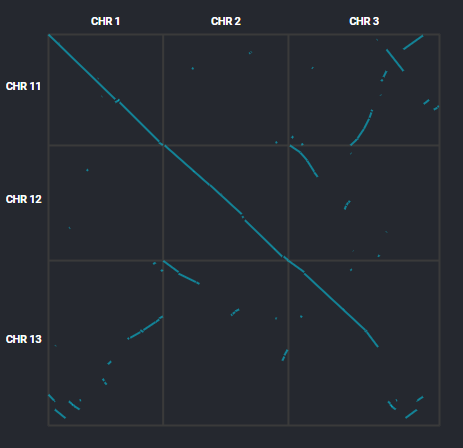
\includegraphics[width=.75\linewidth]{images/ch_1_dot_plot.PNG}
  \captionof{figure}{Dot plot}
  \label{fig:ch_1_dot_plot}
\end{minipage}%
\begin{minipage}{.5\textwidth}
  \centering
  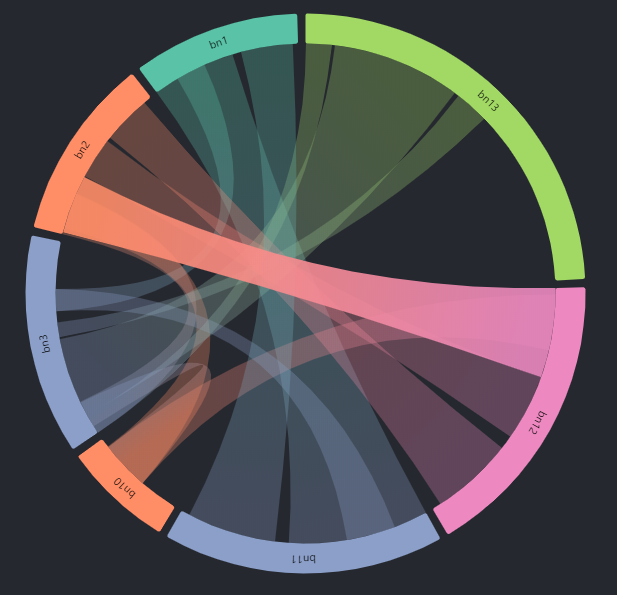
\includegraphics[width=.75\linewidth]{images/ch_1_circos_plot.PNG}
  \captionof{figure}{Circos Plot}
  \label{fig:ch_1_circos_plot}
\end{minipage}
\end{figure}


\section{Problem and Motivation}

The problem addressed in this thesis is: \textit{existing genomic visualizations tools have limited support for exploration, interaction, and collaboration tasks with large scale genomic datasets and are poorly integrated with existing synteny detection tools.}

Understanding genomic conservation is crucial for researchers as it has applications in a wide variety of scenarios, such as predicting whole-genome duplication events, annotating extremely large genome sequences like wheat, and classifying the proximity of different species in their evolutionary history. The increasing size and complexity of genome sequences mean that the work that genomic scientists do with their datasets is constantly evolving: genome visualization tools are now used in diverse tasks such as evolutionary investigations of gene duplication events \cite{rubin2000comparative}, missions to look for new medical treatments \cite{collins2003vision}, and comparisons of gene expression to relate genotype and phenotype \cite{hanada2008importance}. These kinds of complex tasks mean that researchers need access to systems that can support a wide variety of exploration, interaction, and collaboration activities -- and the increasing need for interactivity coupled with the easy availability of datasets (e.g., through public databases such as NCBI and Ensembl) has led to a surge in the demand for computer-based support tools. However, current tools for visualizing and exploring genomic datasets have not kept pace with this increasing demand and are limited in their capabilities: they typically support only a small variety of datasets; they are not designed for investigation of complex synteny scenarios such as polyploidy (whole-genome duplication, which is common in plants); and they often do not support visualizations at multiple genomic scales. A possible reason for these limitations is that genomic visualization tools are rarely developed in close collaboration with the genomic scientists who actually use those tools, and as a result they do not consider the kinds of genomic exploration and analysis tasks that are now performed. For example, a task such as tracing the conservation of genes across more than one species requires the ability to explore pairwise comparisons at multiple levels; similarly, refining sequence assemblies requires annotating existing visualizations with gene density plots to verify assembly quality. 



% refer vgsc

\section{Solution}

\begin{figure}
  \centering
  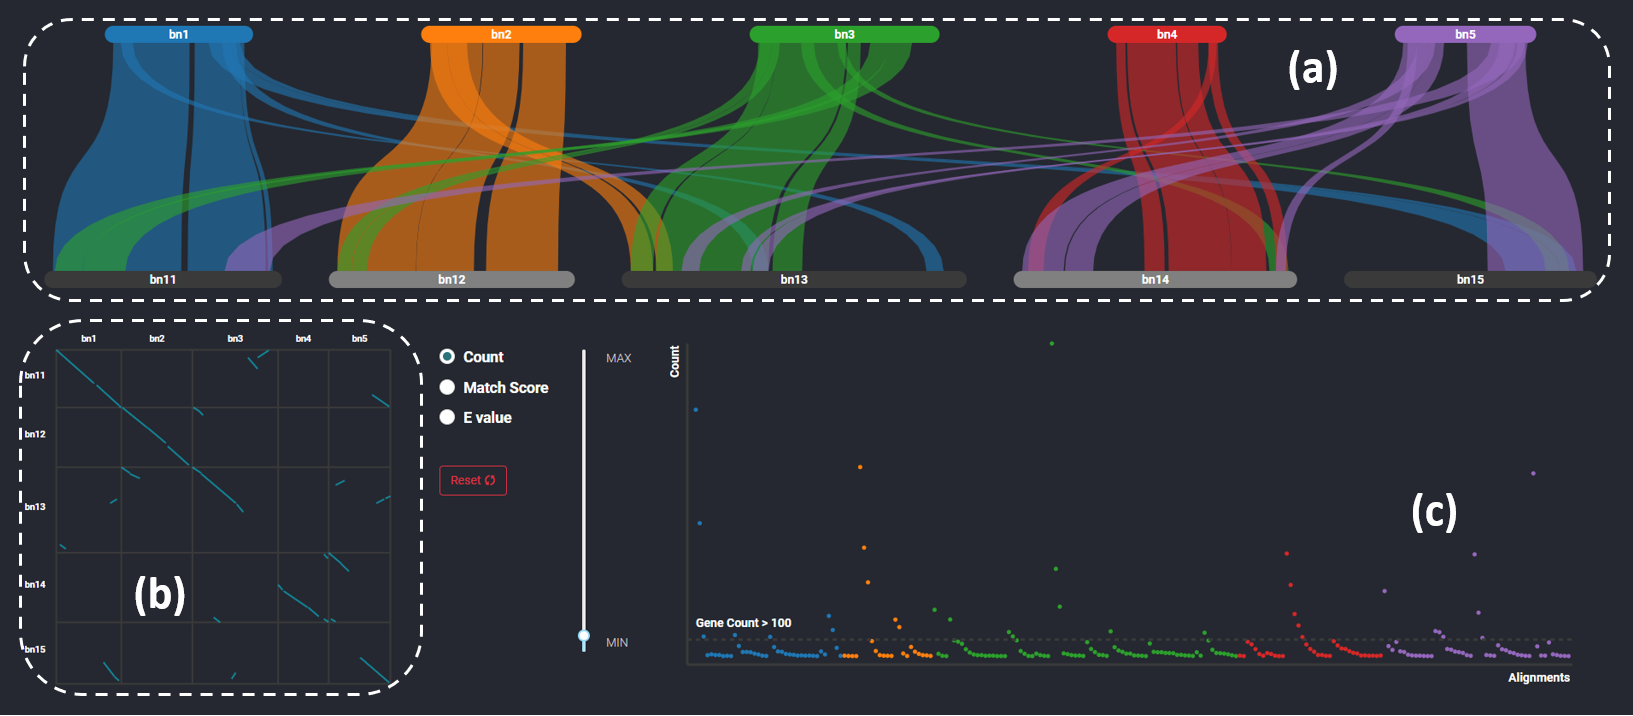
\includegraphics[width=1\linewidth]{images/ch_1_dashboard.PNG}
  \captionof{figure}{Syteny Dashboard visualizing genome collinearity in Bn (Brassica Napus) with the following components: \textbf{a)} Parallel plot with connected ribbons representing collinear gene blocks. \textbf{b)} Dot plot where every collinear gene is represented by a point and contiguous collinear blocks are shown as lines. \textbf{c)} Filter panel representing all the collinear blocks based on the count of their genes with ability to refine results using slider to the left.  }
  \label{fig:ch_1_dashboard}
\end{figure}

To address the limitations of current visualization tools, we met with three teams of genome researchers to understand the interactive and visual requirements for current genomic investigations. The three teams all study plants, but perform very different kinds of exploration and analysis. In collaboration with these experts, we first identified the basic visual requirements of a synteny analysis tool and then supplemented  this list with additional requirements for interactive genomic visualizations that are not supported by current synteny visualization tools such as: the need to refine datasets in real-time, the need to work with multiple perspectives on the data, the need for dynamic multi-resolution visualizations, the need to link secondary datasets to the genomic data, the need for new visualization of synteny across multiple genomes, and the need to support navigation and revisitation in genomic data spaces.

Based on these requirements, we designed a tool called SynVisio that has novel visualization and interaction capabilities to meet the needs of genomics experts. SynVisio is a free web-based system available at \url{https://synvisio.usask.ca}. It lets researchers explore syntenic blocks through coordinated multiple views including parallel plots at several scales (Figure \ref{fig:ch_1_dashboard} (a)), dot plots (Figure \ref{fig:ch_1_dashboard} (b)), and a dynamic filter panel (Figure \ref{fig:ch_1_dashboard} (c)) where users can refine the display of conserved regions based on similarity and the number of contiguous genes in a conserved block.

SynVisio can directly work with the results of existing synteny detecting tools like MCScanX\cite{wang2012mcscanx} and DAGChainer\cite{haas2004dagchainer} and can visualize conservation in multiple representations. SynVisio has two modes: a primary mode, and a multi-analysis mode. Te primary analysis mode lets users compare chromosomes in the same genome or between two genomes, and the information is visualized as parallel plots, dot plots, or both as shown in Figure \ref{fig:ch_1_dashboard}. For visualizing synteny across several genomes simultaneously SynVisio offers a multi-genome analysis mode where synteny is visualized in stacked parallel plots or hive plots. SynVisio further offers a rich interactive experience by letting users switch views in real time and explore data from the genome level all the way down to the individual gene level. Users can do this by simply clicking on any two chromosomes when looking at the visualization in the genome level and then further step down from the individual chromosome level by clicking on a particular gene block to look at its constituent genes and their orientation. Additionally, users can also annotate their views with additional genomic data in the form of tracks above the genomes or chromosomes, which can be visualized as heatmaps, histograms or scatterplots.

As exploration in SynVisio is heavily based on user interactions, it offers them the ability to record these interactions as snapshots, for future revisitation. This gives users the ability to examine multiple scenarios and rapidly switch between them in real-time. The system also indexes all the conserved genes in the browser, thus letting users quickly look up genes by their gene IDs to see which conserved blocks they belong to. Finally, SynVisio offers users the ability to download all generated visualizations in transform and scale invariant vector graphics for research publications.

\section{Steps to the Solution} 
There were several steps involved in designing a system that addressed the usability issues mentioned in the problem statement.

\begin{itemize}
    
    \item \textbf{Formulate Design Requirements} -
    To characterize the needs from the biological research community, we primarily met with three groups of researchers studying genomic conservation through a series of structured interviews to collect their requirements. The first group we met was interested in exploring synteny in wheat while the other two groups were involved in studying canola and pulse crops respectively. All three groups were unanimous in the verdict that synteny is a critical issue to study for understanding genomic evolution and that existing tools don't meet their needs. Based on the feedback from the genomic research community all requirements can be broadly classified into either \textbf{functional} or \textbf{supplementary} requirements. Functional requirements primarily include understanding the size, location, and orientation of conserved sequences along with having the ability to filter sequences based on their similarity while non-functional requirements include features like the ability to download images or snapshot explorational points to revisit.
    
    \item \textbf{Identify and Explore Existing Alternatives} - 
    Since synteny analysis is a combination of synteny detection followed by downstream analysis using visualization systems, we looked at tools that operate in both these domains. We looked at several state of the art syteny detection packages like MCScanX, DAGChainer, Cyntenator and i-ADHoRe \cite{wang2012mcscanx,haas2004dagchainer,rodelsperger2010cyntenator,proost2011adhore}. We also tested the visual outputs of some that had their own downstream analysis tools. We focused our research on MCScanX and DAGChainer out of the other alternatives as they were the most popular and frequently used tools by the researchers we interviewed and had more accessible and  efficient output data formats in the form of syntenic blocks or orthologue tables. We followed this by looking at the tools that worked in the second stage of the analysis pipeline by providing visualizations, like SynChro, GSV, Mizbee, VGSC, and Circos\cite{drillon2014synchro,revanna2011gsv,Meyer2009,xu2016vgsc}. Of these, we found that most served as simple graphic generating systems instead of offering a platform for detailed analysis except for MizBee, which was however, limited by its accessibility and small variety of charts.

    \item \textbf{Explore Visual Design and Architecture} - 
    To implement our solution, we decided on a web-based single page tool that would work as a part of the existing analysis pipeline by working directly on the results of existing synteny detection tools. We adopted a thick-client architecture model instead of the traditional thin client model where visualizations are generated on the server, as a thick-client model would let researchers directly upload their analysis files and see the resulting images in real time without their sensitive data being sent to a remote server. To visually represent genomic conservation, we used linear connections (parallel plots) and points (dot plots). We then encoded additional information about the size and orientation of the gene blocks through a combination of colour and shape.
   
   \item \textbf{Implement System} - We built SynVisio using a combination of React.JS\cite{react} and D3.JS\cite{d3js}. The former was used to render the visual elements on the web interface while the latter was used to calculate the positions of the graphical elements. To render the visualizations, we used both canvas and simple vector graphics (SVG) and compared their performance. We found that vector graphics based visualizations while being more resource intensive offered a better visual experience across different resolutions with greater scope for interactive features. So our system was designed to render all charts as simple vector graphics by default but can dynamically switch to canvas for rendering of large scale genomes when there are a large number of individual graphics elements. The final application was developed through several design iterations as the system was used by members of our expert user group and several additional features such as support for additional tracks and the ability to download publication ready images were added based on their feedback. 

\end{itemize}

\section{Evaluation}

A stable version of SynVisio was deployed and has been available for public use since the start of 2019. Evaluation of our system was done in two ways: a log based usage study and an interview-based expert study. Firstly to determine the overall use of our system, we analyzed the web traffic logs to SynVisio for a period of one year (2019-2020). We found that it had 154 unique visitors from 18 different countries across the world using it for a wide variety of projects. Additionally, during this period, the open-sourced code for SynVisio was made available on GitHub under a free MIT License and has since been adopted into several online genome databases for species such as Tea, Grape Vine, and Silkworm respectively.

To see if we had met our design requirements, we also evaluated our system through semi-structured interviews with five domain experts consisting of four genome researchers and one bioinformatician. The interviews were conducted via phone or in person and lasted around 45-60 minutes. Researchers were asked open-ended questions about synteny analysis and how it is used in their field of research. They were then asked to give their opinion on the various features of the system that were developed to improve its usability. Finally they were also asked to rate the ability of the system to visualize genomic conservation on a scale of 1 (very bad) to 5 (very good), and four researchers gave the system 5/5, and one researcher gave the system 4/5. The positive feedback from our user study, coupled with the broad usage of the system from researchers around the world, shows that SynVisio has been able to address the problem of limited usability of synteny analysis tools.

\section{Thesis Outline}

This thesis is organized into eight chapters, including the current chapter. Chapter 2 firstly present a discussion of the biological background behind genomic conservation and synteny in particular and looks at the different ways in which studying such conservation can assist researchers. We then explore the framework of synteny detection and some of the tools that are currently being used. Secondly, we look at the different kinds of visualization systems and techniques that are used in representing genomic data at various resolutions. We then look at visualization systems dedicated to analyzing sequence similarity and synteny and discuss their merits and limitations. Finally, we explore the various techniques that genomic visualization tools utilize to manipulate both the underlying data and the graphical representation to facilitate data exploration.

In chapter 3, we first discuss the underlying data abstraction layer in our system by describing the properties of syntenic data and how it is computed and processed. We follow this with an exploration of the different analysis tasks that can be performed on syntenic data and organize these tasks into three basic groups according to the genomic scale at which they operate. We finally discuss supplementary requirements that can enhance user experience with the system.

 Chapter 4 provides a discussion of the visual design of SynVisio. We first explore the different forms of visual encoding used in representing genomic conservation and follow this with a description of the different layout strategies that were explored in designing SynVisio. We then discuss the interaction strategies that were adopted in our final design based on the visual information seeking mantra framework and design of multiple coordinated views. Finally, we conclude the chapter with a summary of the various steps in our iterative design cycle.

Chapter 5 presents a detailed description of our visualization system SynVisio. We first discuss the different modes of synteny analysis SynVisio offers and how they operate. We then provide a description of the various supplementary features that SynVisio provides to enhance user experience with the tool. Finally, we elaborate on the choices made in the architecture of the system,
and discuss the software implementation of SynVisio as a web interface built with JavaScript.

Chapter 6 provides a detailed evaluation of our system. To quantify user engagement, web traffic to the system was analyzed for a period of one year. Examples of adaptations of open-sourced code of SynVisio in several online genome databases are also discussed. Finally, a user study was conducted with five researchers through semi-structured interviews, and their responses are summarized through three major case studies highlighting the usability of our system across different types of genomes.

Chapter 7 presents a discussion of the design choices and the insight gained from the development of our genomic visualization system. Further, it also presents the current limitations of our system and highlights possible avenues for improvement in the future.

Finally, Chapter Eight summarizes this thesis. It reiterates the problem statement and outlines our major contributions.